\documentclass[usenames,dvipsnames,modern]{CLASS_FILES/aastex631}
\usepackage{CLASS_FILES/FUpackages}  % applying Frequently-Used packages
\usepackage{CLASS_FILES/FUformatting} % apply Frequently-used formatting definitions/setups
\usepackage{CLASS_FILES/FUnewCommands} % apply Frequently-used usercommands

%....................................
% additonal items specific to this document
\fancyhead[L]{\color{WatermarkColor}EXAMPLES}
\fancyhead[R]{\color{WatermarkColor}All of the \texttt{WorPT} Tables}
%....................................

%      S T A R T  D O C U M E N T 
\begin{document}

\tableofcontents
\addtocontents{toc}{~\hfill\textbf{Page}\par}
\pagenumbering{roman}
\newpage
\pagenumbering{arabic}

\section{What Is This Document?}
This document illustrates what each table generated from the \texttt{WorPT} (Work Plan Tool for proposals) tool looks like when rendered.  Use the Table of Contents to quickly jump to a table of interest.  The file name corresponding to each table is provided for easy reference. 

Note that the table files are not stagnant; they will change with time as we evolve our preferences, and as we identify other tables to add to the list of files generated by \texttt{WorPT}.  To incorporate the latex table files, \emph{ALWAYS} use the instructions provided at the top of the latex file in the commented region, as those instructions may also change over time (see snapshot of an example of such instructions below.  To use the file in a document, all you do is uncomment-out the lines under #2, see yellow highlight: 

\begin{figure}[h]
    \centering
    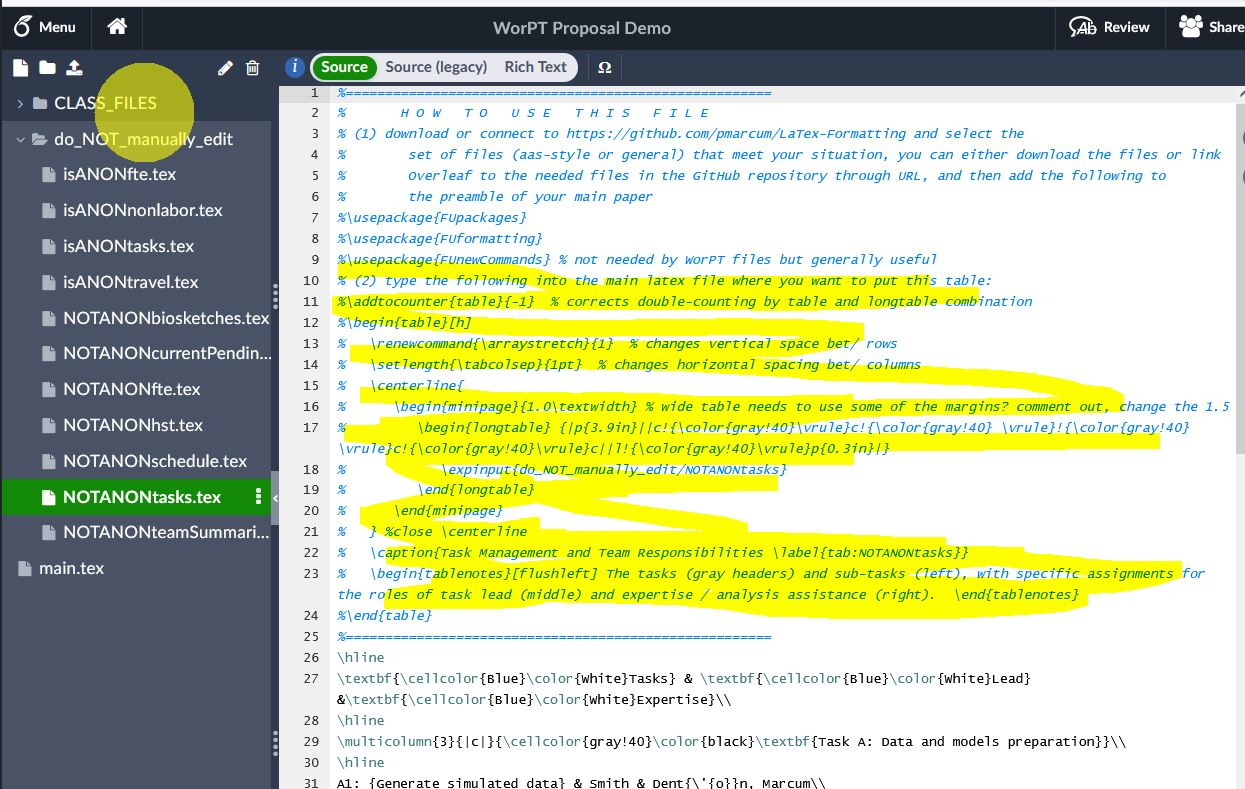
\includegraphics[width=0.98\textwidth]{latexFileInstructions.JPG}
    \caption{Example of the instructions at the top of the \texttt{WorPT} table files.}
    \label{fig:latexFileExample}
\end{figure}

Red-colored font appearing in the following table examples indicate captions, descriptions, etc. that will likely need to be edited so that the words match the proposal or paper being worked on. 

The most recent version of the \href{https://docs.google.com/spreadsheets/d/1J9svcoISn2EjHlWNVp2gkKhlgJeGj1BwTQ4coAc9_8E/edit#gid=901021069}{\texttt{WorPT} is here.} A clean GitHub version will be available soon, and should be the starting point for any new proposal, to ensure that the latest version is being used, and that old info isn't accidentally carried over into the new project.  Note that rows are now added to both the Personnel and the Tasks sheets by simply adding the rows the usual "Google Sheet" way, rather than having to hit a button! 

% @@@@@@@@@@@@@@@@@@@@@@@@@@@@@@@@@@@@@@@@@@@@@@@@@@@@@@@@@@@@@@@@@@@@@@@@@@@@@@@
% @@@@@@@@@@@@@@@@@@@@@@ F T E s   P E R   P E R S O N  @@@@@@@@@@@@@@@@@@@@@@@@@
% @@@@@@@@@@@@@@@@@@@@@@@@@@@@@@@@@@@@@@@@@@@@@@@@@@@@@@@@@@@@@@@@@@@@@@@@@@@@@@@
\newpage
\mbox{} \vfill \section{FTEs PER PERSON INFORMATION} \vfill \mbox{}

% ___________________________________________________
%     A N O N O N Y M O U S   F T E
% ___________________________________________________
\newpage
\subsection{\textbf{Anonymous} FTEs per Year per Team Member Role (``isANONfte.tex'')}
{
   \renewcommand{\arraystretch}{1.0} %adjust to control vertical row separation/spacing, comment-out if not needed
   \setlength{\tabcolsep}{5pt} %adjust to control horizontal column separation/spacing, comment-out if not needed
   \begin{longtable}{|l|*{4}{c|}}
      \expinput{do_NOT_manually_edit/isANONfte}
      \caption{\label{tab:isANONfte} Details of work efforts per member to be funded for the present proposal; {\color{red}Detailed responsibilities, tied to tasks and science goals, are provided in Sec.\,\ref{Subsec:tmeline}.}}
   \end{longtable}
}

% ___________________________________________________
%    N O T  A N O N O N Y M O U S   F T E 
% ___________________________________________________
\newpage
\subsection{\textbf{Not} Anonymous FTEs per Year Per Named Team Member Role  (``NONANONfte.tex'')}
{
   \renewcommand{\arraystretch}{1.0} %adjust to control vertical row separation/spacing, comment-out if not needed
   \setlength{\tabcolsep}{5pt} %adjust to control horizontal column separation/spacing, comment-out if not needed
   \begin{longtable}{|l|l|*{4}{c|}}
      \expinput{do_NOT_manually_edit/NOTANONfte}
      \caption{\label{tab:NOTANONfte} FTE/WYE for all team members.}
   \end{longtable}
}

% ___________________________________________________
%   N O T  A N O N O N Y M O U S  H S T - S T Y L E 
% ___________________________________________________
\newpage
\subsection{\textbf{Not} Anonymous HST-style FTE Table for Phase~II (``NOTANONhst.tex'')}
% Block of code to be uncommented by removing the *first* percent-sign at the beginning of the following lines below (leave intentional comments with at least 1 percent sign to keep them commented!)
% The next couple of lines define cell and font colors that can be changed if desired (keep this comment line commented-out!)
\def\myHeaderColor{Blue} % Color of column headings
\def\myLabelColor{White} % Color of font column headings
\def\myLabelBoldface#1{\textbf{#1}} % Makes column labels bold-faced; change {\textbf{#1}} to {#1} or to other preference.
%
\newcolumntype{L}[1]{>{\raggedright\let\newline\\\arraybackslash\hspace{0pt}}p{#1}}
{
   \renewcommand{\arraystretch}{1.0} %adjust to control vertical row separation/spacing, comment-out if not needed
   \setlength{\tabcolsep}{5pt} %adjust to control horizontal column separation/spacing, comment-out if not needed
   \begin{longtable}{
      |L{1.8in}!{\color{lightgray}\vrule}L{1.3in}!{\color{lightgray}\vrule}L{2.5in}!{\color{lightgray}\vrule}p{0.10in}!{\color{lightgray}\vrule}p{0.28in}|
      }
      \caption{Work Effort for All Team Members \label{tab:NOTANONhst}}\\
      \multicolumn{5}{l}{\textbf{Program \#:} HST-xx-xxxxx (Cycle XX)}\\

      \multicolumn{5}{l}{\textbf{Science PI:} Dr. Sally Smith}\\
      \expinput{do_NOT_manually_edit/NOTANONhst}
   \end{longtable}
}

% @@@@@@@@@@@@@@@@@@@@@@@@@@@@@@@@@@@@@@@@@@@@@@@@@@@@@@@@@@@@@@@@@@@@@@@@@@@@@@@
% @@@@@@@@@@@@@@@@@@@@@@ T A S K S   &   S C H E D U L E S @@@@@@@@@@@@@@@@@@@@@@
% @@@@@@@@@@@@@@@@@@@@@@@@@@@@@@@@@@@@@@@@@@@@@@@@@@@@@@@@@@@@@@@@@@@@@@@@@@@@@@@
\newpage
\mbox{} \vfill \section{TASKS \& SCHEDULES} \vfill \mbox{}

% ___________________________________________________
%           I S  A N O N   t a s k s
% ___________________________________________________
\newpage
\subsection{\textbf{Anonymous} Task Start/Finish vs Role Assignment (``isANONtasks.tex'')}
\addtocounter{table}{-1} % corrects double-counting of longtable and table combination
\begin{table*}[h!] %table is needed so that table caption at bottom has same width as table
   \renewcommand{\arraystretch}{0.7} %adjust to control vertical row separation/spacing
   \setlength{\tabcolsep}{5pt} %adjust to control horizontal column separation/spacing
   \begin{longtable}{|p{3.3in}||c!{\color{lightgray}\vrule}c!{\color{lightgray}\vrule}!{\color{lightgray}\vrule}c!{\color{lightgray}\vrule}c||p{0.45in}!{\color{lightgray}\vrule}p{1.2in}|}
      \expinput{do_NOT_manually_edit/isANONtasks}
   \end{longtable}
   \caption{\label{tab:isANONtasks} \textbf{Task Timeline:} Team member roles, rightmost column, are cross-referenced with corresponding names in the non-anonymized personnel and work effort table.  {\color{red} \textbf{Paper~1:} Sample and methods for enhancing detectability of  low SB X-ray emission, presentation of emission maps, description of database and pipeline software (which will be released in a public repository at the time of paper submission). \textbf{Paper~2:} Methodologies for measuring the gas halo size and other gas properties, analyisis of the diffuse hot gas halos as functions of galaxy properties (environment, galaxy morphology, stellar mass, and SFR based on \Chandra, \Hubble, and \Spitzer\ observations, and the SED models from the GSWLC; application of multivariate mthods to ``baseline'' the gas halo sizes (Sect.\,\ref{Sec:Baseline}). \textbf{Note~1:} See Sec.\,\ref{Sec:Sample}.}}
\end{table*}

% ___________________________________________________
%           N O T  A N O N   t a s k   s c h e d u l e
% ___________________________________________________
\newpage
\subsection{\textbf{Not} Anonymous Detailed Resource-Loaded Task Timeline w/ Assignments (``NOTANONschedule.tex'')}
\addtocounter{table}{-1} %corrects double-counting of sidewaystable and longtable combination
%\begin{sidewaystable}  %comment out if not needed
   \begingroup
      \setlength{\tabcolsep}{1pt}  % changes horizontal spacing between columns
      \renewcommand{\arraystretch}{0.8} %changes vertical space between rows
      \centerline{
         \begin{minipage}{1.5\textwidth}  %wide table needs some of the margin?  change 1.5 to whatever
            \begin{longtable} {|>{\raggedright\arraybackslash}p{3.1in} % title column
               *{3}{|p{1ex}!{\color{lightgray}\vrule}*{2}{p{1ex}!{\color{lightgray}\vrule}}p{1ex}}%year
               |>{\raggedright\arraybackslash}p{20ex}%task assignments (ID and \#Weeks)
               |p{5ex}!{\color{lightgray}\vrule}p{5ex}!{\color{lightgray}\vrule}c|%TOTAL FTE columns
               }
               \expinput{do_NOT_manually_edit/NOTANONschedule}
            \end{longtable}
         \end{minipage}
      }
   \endgroup
   \caption{\label{tab:NOTANONschedule} Resource-loaded project schedule, where: {\raisebox{-0.3\normalbaselineskip}[0pt][0pt]{
\begin{tikzpicture} \draw[fill=white,draw=red,line width=0.4mm] (0,0) circle[radius=0.2]; \draw[line width=0.4mm,red] node[midway,black]{\faDollar} (0.15,0.15) -- (-0.15,-0.15);  \draw[line width=0.4mm,red] (0.15,0.15) -- (-0.15,-0.15);  \end{tikzpicture}}} Not funded by this grant,  {\raisebox{-0.3\normalbaselineskip}[0pt][0pt]{
\begin{tikzpicture}  \draw[fill=green,draw=black] (0,0) circle[radius=0.2];  \draw[draw=green] (-0.015,0.015) -- (0.015,-0.015) node[midway]{\faDollar};  \end{tikzpicture}}} funded by this grant, {\textbf{\large{$\Sigma$}}} funded $+$ unfunded; Tasks are listed (left side), with duration of task activity indicated in blue-colored timelines  that measure quarter-years (1,2,3,4). Task assignments identify specific team members responsible for  implementation with associated work weeks, where color indicates institutional affiliation  (blue$=$funded/U.S., black$=$not funded/U.S., red=international). "Total FTE" (right side) are integrated work-weeks converted into FTE per task (1~FTE$=$12~months), displayed as "total",  "unfunded by this grant", and "funded by this grant", resp.  Asignment identities:  {\textbf{dd}}: Dan.Dent{\'{o}}n, {\textbf{gg}}: Gisella.Gala, {\textbf{pm}}: Pamela.Marcum, {\textbf{ss}}: Sally.Smith}
%\end{sidewaystable}  % comment out if not used

% @@@@@@@@@@@@@@@@@@@@@@@@@@@@@@@@@@@@@@@@@@@@@@@@@@@@@@@@@@@@@@@@@@@@@@@@@@@@@@
% @@@@@@@@@@@@@@@@@ T A S K   A S S I G N M E N T S @@@@@@@@@@@@@@@@@@@@@@@@@@@@
% @@@@@@@@@@@@@@@@@@@@@@@@@@@@@@@@@@@@@@@@@@@@@@@@@@@@@@@@@@@@@@@@@@@@@@@@@@@@@@
\newpage
\mbox{} \vfill
\section{TASK ASSIGNMENTS}
\vfill \mbox{}
Also see TABLE\,\ref{tab:isANONtasks} and \ref{tab:NOTANONschedule}

% ___________________________________________________
%           N O T  A N O N   t a s k s
% ___________________________________________________
\newpage
\subsection{\textbf{Not} Anonymous Simple Task List w/ Named Team Responsibilities (no FTEs) (``NOTANONtasks.tex'')}
\def\myHeaderColor{Blue} % Color of column headings
\def\myLabelColor{White} % Color of font column headings
\def\myLabelBoldface#1{\textbf{#1}} % Makes column labels bold-faced; change {\textbf{#1}} to {#1} or to other preference.
\def\mySectionColor{gray!40} % Color of section labels giving the Task category names, e.g., "Task A: ...."
\def\myTaskColor{Black} % Color of task category label, e.g. "Task A: ...."
\def\myTaskBoldface#1{\textbf{#1}} % Makes the task category labels bold-faced; change {\textbf{#1}} to {#1} or to other preference.
%
\addtocounter{table}{-1}  % corrects double-counting by table and longtable combination
\begin{table}[h]
   \renewcommand{\arraystretch}{1}  % changes vertical space bet/ rows
   \setlength{\tabcolsep}{1pt}  % changes horizontal spacing bet/ columns
   \centerline{
      \begin{minipage}{1.0\textwidth} % wide table needs to use some of the margins? comment out, change the 1.5
         \begin{longtable} {|p{3.9in}||c!{\color{gray!40}\vrule}c!{\color{gray!40} \vrule}!{\color{gray!40}\vrule}c!{\color{gray!40}\vrule}c||l!{\color{gray!40}\vrule}p{0.3in}|}
            \expinput{do_NOT_manually_edit/NOTANONtasks}
         \end{longtable}
      \end{minipage}
   } %close \centerline
  \caption{Task Management and Team Responsibilities \label{tab:NOTANONtasks}}
  \begin{tablenotes}[flushleft] The tasks ({\color{red}gray} headers) and sub-tasks (left), with specific assignments for the roles of task lead (middle) and expertise / analysis assistance (right).  \end{tablenotes}
\end{table}

% _____________________________________________________________________
%     N O T  A N O N   t e a m   s u m m a r y  n a r r a t i v e s
% _____________________________________________________________________
\newpage
\subsection{\textbf{Not} Anonymous Team Summary Role Descriptions  (``NOTANONteamSummaries.tex'')}
%\clearpage
%======================================================
%     H O W   T O   U S E   T H I S   F I L E
% (1) download or connect to https://github.com/pmarcum/LaTex-Formatting and select the
%        set of files (aas-style or general) that meet your situation, you can either download the files or link
%        Overleaf to the needed files in the GitHub repository through URL, and then add the following to
%        the preamble of your main paper
%\usepackage{FUpackages}
%\usepackage{FUformatting}
%\usepackage{FUnewCommands} % not needed by WorPT files but generally useful
% (2) type the following into the main latex file where you want to put this section of text (it is not a table):
%\clearpage
%%======================================================
%     H O W   T O   U S E   T H I S   F I L E
% (1) download or connect to https://github.com/pmarcum/LaTex-Formatting and select the
%        set of files (aas-style or general) that meet your situation, you can either download the files or link
%        Overleaf to the needed files in the GitHub repository through URL, and then add the following to
%        the preamble of your main paper
%\usepackage{FUpackages}
%\usepackage{FUformatting}
%\usepackage{FUnewCommands} % not needed by WorPT files but generally useful
% (2) type the following into the main latex file where you want to put this section of text (it is not a table):
%\clearpage
%%======================================================
%     H O W   T O   U S E   T H I S   F I L E
% (1) download or connect to https://github.com/pmarcum/LaTex-Formatting and select the
%        set of files (aas-style or general) that meet your situation, you can either download the files or link
%        Overleaf to the needed files in the GitHub repository through URL, and then add the following to
%        the preamble of your main paper
%\usepackage{FUpackages}
%\usepackage{FUformatting}
%\usepackage{FUnewCommands} % not needed by WorPT files but generally useful
% (2) type the following into the main latex file where you want to put this section of text (it is not a table):
%\clearpage
%\input{do_NOT_manually_edit/NOTANONteamSummaries}
%======================================================
Dr. \textbf{Dan J. Dent{\'{o}}n, III}, \textbf{PI}, will lead the emission maps production, and the reduction of image mosaics related to archive applications. Finally, he will lead the first publication, a paper describing the pipeline and improved images.  His $\sim$15 years of experience in image analysis are needed for successful and timely completion of these tasks. In addition to leading these tasks, he will assist with model preparation by generating simualted data, and will identify fields of interest for the archive-related work, as well as help with code documentation and the development of the second publication. \par
Dr. \textbf{Sally K. Smith}, \textbf{Sci-PI}, will lead simulated data generation for models input and the incorporation of thermal models, as well as code documentation.  Her extensive work with model simulations and archival processes are well-matched to these roles.  Additionally, her expertise will be used to assist with generation of emission maps, identifying fields of interest, reduction of image mosaics and in the development of both publications. \par
Dr. \textbf{Pamela M. Marcum}, \textbf{co-I(1)}, will lead the identification of fields and the second publication, a paper on galaxy identification.  Her background in extragalactic astronomy is essential for successful implementation of these tasks. In addition to these responsibilities, she will provide expertise in the model preparation by generating simulated input data, and in the incorporation of thermal emission models.  She will also assist with documentation and will co-author the first publication. \par
%======================================================
Dr. \textbf{Dan J. Dent{\'{o}}n, III}, \textbf{PI}, will lead the emission maps production, and the reduction of image mosaics related to archive applications. Finally, he will lead the first publication, a paper describing the pipeline and improved images.  His $\sim$15 years of experience in image analysis are needed for successful and timely completion of these tasks. In addition to leading these tasks, he will assist with model preparation by generating simualted data, and will identify fields of interest for the archive-related work, as well as help with code documentation and the development of the second publication. \par
Dr. \textbf{Sally K. Smith}, \textbf{Sci-PI}, will lead simulated data generation for models input and the incorporation of thermal models, as well as code documentation.  Her extensive work with model simulations and archival processes are well-matched to these roles.  Additionally, her expertise will be used to assist with generation of emission maps, identifying fields of interest, reduction of image mosaics and in the development of both publications. \par
Dr. \textbf{Pamela M. Marcum}, \textbf{co-I(1)}, will lead the identification of fields and the second publication, a paper on galaxy identification.  Her background in extragalactic astronomy is essential for successful implementation of these tasks. In addition to these responsibilities, she will provide expertise in the model preparation by generating simulated input data, and in the incorporation of thermal emission models.  She will also assist with documentation and will co-author the first publication. \par
%======================================================
Dr. \textbf{Dan J. Dent{\'{o}}n, III}, \textbf{PI}, will lead the emission maps production, and the reduction of image mosaics related to archive applications. Finally, he will lead the first publication, a paper describing the pipeline and improved images.  His $\sim$15 years of experience in image analysis are needed for successful and timely completion of these tasks. In addition to leading these tasks, he will assist with model preparation by generating simualted data, and will identify fields of interest for the archive-related work, as well as help with code documentation and the development of the second publication. \par
Dr. \textbf{Sally K. Smith}, \textbf{Sci-PI}, will lead simulated data generation for models input and the incorporation of thermal models, as well as code documentation.  Her extensive work with model simulations and archival processes are well-matched to these roles.  Additionally, her expertise will be used to assist with generation of emission maps, identifying fields of interest, reduction of image mosaics and in the development of both publications. \par
Dr. \textbf{Pamela M. Marcum}, \textbf{co-I(1)}, will lead the identification of fields and the second publication, a paper on galaxy identification.  Her background in extragalactic astronomy is essential for successful implementation of these tasks. In addition to these responsibilities, she will provide expertise in the model preparation by generating simulated input data, and in the incorporation of thermal emission models.  She will also assist with documentation and will co-author the first publication. \par

% @@@@@@@@@@@@@@@@@@@@@@@@@@@@@@@@@@@@@@@@@@@@@@@@@@@@@@@@@@@@@@@@@@@@@@@@@@@@@@
% @@@@@@@@@@@@@@@@@   B I O G R A P H I C A L   I N F O  @@@@@@@@@@@@@@@@@@@@@@@
% @@@@@@@@@@@@@@@@@@@@@@@@@@@@@@@@@@@@@@@@@@@@@@@@@@@@@@@@@@@@@@@@@@@@@@@@@@@@@@
\newpage
{\mbox{} \vfill \section{BIOGRAPHICAL INFORMATION ON TEAM MEMBERS} \vfill \mbox{}}

% _____________________________________________________________________
%        N O T  A N O N Y M O U S   b i o s k e t c h e s 
% _____________________________________________________________________
\newpage
\subsection{\textbf{Not} Anonymous Biographical Sketches (``NOTANONbiosketches.tex'')}
%\clearpage  % or you might want to use \newpage or \pagebreak, whatever works best
%======================================================
%     H O W   T O   U S E   T H I S   F I L E
% (1) download or connect to https://github.com/pmarcum/LaTex-Formatting and select the
%        set of files (aas-style or general) that meet your situation, you can either download the files or link
%        Overleaf to the needed files in the GitHub repository through URL, and then add the following to
%        the preamble of your main paper
%\usepackage{FUpackages}
%\usepackage{FUformatting}
%\usepackage{FUnewCommands} % not needed by WorPT files but generally useful
% (2) type the following into the main latex file where you want to put this section of text (it is not a table):
%\clearpage  % or you might want to use \newpage or \pagebreak, whatever works best
%%======================================================
%     H O W   T O   U S E   T H I S   F I L E
% (1) download or connect to https://github.com/pmarcum/LaTex-Formatting and select the
%        set of files (aas-style or general) that meet your situation, you can either download the files or link
%        Overleaf to the needed files in the GitHub repository through URL, and then add the following to
%        the preamble of your main paper
%\usepackage{FUpackages}
%\usepackage{FUformatting}
%\usepackage{FUnewCommands} % not needed by WorPT files but generally useful
% (2) type the following into the main latex file where you want to put this section of text (it is not a table):
%\clearpage  % or you might want to use \newpage or \pagebreak, whatever works best
%%======================================================
%     H O W   T O   U S E   T H I S   F I L E
% (1) download or connect to https://github.com/pmarcum/LaTex-Formatting and select the
%        set of files (aas-style or general) that meet your situation, you can either download the files or link
%        Overleaf to the needed files in the GitHub repository through URL, and then add the following to
%        the preamble of your main paper
%\usepackage{FUpackages}
%\usepackage{FUformatting}
%\usepackage{FUnewCommands} % not needed by WorPT files but generally useful
% (2) type the following into the main latex file where you want to put this section of text (it is not a table):
%\clearpage  % or you might want to use \newpage or \pagebreak, whatever works best
%\input{do_NOT_manually_edit/NOTANONbiosketches}
%================ E N D   I N S T R U C T I O N S ===============
\textbf{\color{Blue}\large Dr. Daniel Dent{\'o}n (Principal Investigator):}\\
University of CBA\\
\vspace{4ex}
\textbf{Education}\\
01012004 - 12312008, University of ABC, Ph.D., astrophysics\\
01012000 - 12312003, University of XYZ, B.S., astronomy\\
\textbf{Appointments}\\
01012012 - present, professor, University of CBA\\
01032009 - 01082011, postdoc, University of ZYX\\
\textbf{Additional Awards, Positions, Fellowships and Proposals}\\
01102011 - 01102012, Awarded 100 hrs on Gigantic Telescope\\
01052011, Best Researcher of the Year\\
\textbf{Publications relevant for the proposal:}\\
{\scriptsize{$\bullet$}} Young, E.T., Herter, T.L., Gusten, R., et al. (inc. \textbf{Denton, D.}), 2021, "Early science results from SOFIA", 8444, 844410\\
{\scriptsize{$\bullet$}} Temi, P., \textbf{Denton, D.}, Miller, W.E., et al., 2018, "SOFIA observatory performance and characterization", SPIE, 84444, 8444414\\
{\scriptsize{$\bullet$}} Gehrz, R.D., Becklin, E.E., et al. (inc.\textbf{Denton, D.}), 2015, "Status of the Stratospheric Observatory for Infrared Astronomy (SOFIA)", Adv. in Space Research, 48, 1004\\
{\scriptsize{$\bullet$}} \textbf{Denton, D.}, Appleton, P.N., Higdon, J.L, 2010, "Large Infrared and Optical Color Gradients in the Carwheel Ring Galaxy: Evidence fo rthe First Epoch of Star Formation in the Wake of an Expanding Ring", ApJ, 399, 57\\
\medskip \hrule \vspace{5pt} \medskip
\textbf{\color{Blue}\large Dr. Sally Smith (Science PI):}\\
University of CBA\\
\vspace{4ex}
\textbf{Education}\\
01012014 - 12312020, University of lmn, Ph.D., astronomy\\
01012010 - 12312014, University of abc, B.S., physics\\
\textbf{Appointments}\\
01012023 - present, research fellow, University of CBA\\
01032020 - 01082022, postdoc, University of ZYX\\
\textbf{Additional Awards, Positions, Fellowships and Proposals}\\
01102011 - 01102012, Awarded 100 hrs on Gigantic Telescope\\
43332, Teaching assistant award\\
\textbf{Publications relevant for the proposal:}\\
{\scriptsize{$\bullet$}} Lopez-Rodriguez, E., Mao, S.A., Beck, R., et al. (inc. \textbf{Smith, S.}), 2022, "Extragalactic magnetism with SOFIA (SALSA Legacy Program) IV: Program overview and first results on the polarization fraction" (submitted to ApJ)\\
{\scriptsize{$\bullet$}} Young, E.T., Herter, T.L., Gusten, R., et al. (inc. \textbf{Smith, S.}), 2021, "Early science results from SOFIA", 8444, 844410\\
{\scriptsize{$\bullet$}} Gehrz, R.D., Becklin, E.E., et al. (inc.\textbf{Smith, S.}), 2015, "Status of the Stratospheric Observatory for Infrared Astronomy (SOFIA)", Adv. in Space Research, 48, 1004\\
{\scriptsize{$\bullet$}} \textbf{Smith, S.}, Appleton, P.N., Higdon, J.L, 2010, "Large Infrared and Optical Color Gradients in the Carwheel Ring Galaxy: Evidence fo rthe First Epoch of Star Formation in the Wake of an Expanding Ring", ApJ, 399, 57\\
\medskip \hrule \vspace{5pt} \medskip
\textbf{\color{Blue}\large Dr. Pamela M. Marcum (co-Investigator):}\\
NASA ARC\\
\vspace{4ex}
\textbf{Education}\\
1994, University of Wisconsin, Ph.D., Astrophysics\\
1989, Florida Institute of Technology, M.S., Space Science\\
1989, Florida Institute of Technology, M.S., Physics\\
1987, Florida Institute of Technology, B.S., Space Science\\
\textbf{Appointments}\\
2016 - present, research scientist, NASA Ames Research Center\\
2020 - 2021, program officer (on detail), NASA HQ, Washington, D.C.\\
2009 - 2016, SOFIA project scientist, NASA Ames Research Center\\
2005 - 2008, program officer (IPA), NASA HQ, Washington, D.C.\\
2003 - 2009, associate professor, Texas Christian University (Fort Worth, TX)\\
1996 - 2002, assistant professor, Texas Christian University (Fort Worth, TX)\\
1994 - 1996, postdoctoral fellow, University of Virginia\\
\textbf{Additional Awards, Positions, Fellowships and Proposals}\\
2018 - present, Roman Space Telescope Standing Review Board\\
2021 - 2022, SOFIA Cycle 9 observing proposal 09\_0113: "Testing for multi-component magnetic fields and their effects on the structure of galaxtic disks", 20.1h, SOFIA/HAWC+ (pending observations/funding)\\
2021, VLA/21A-043,"Flares, breaks and warps in the outskirts of the HI and stellar disk of UGC11859", 9h, HI observations, JVLA C-array\\
2020, VLA/20A-493, "Clues to the Origin of Cold Gas in the Void Elliptical Galaxy KIG 16", 12h (DDT),HI observations, JVLA C-array\\
\textbf{Publications relevant for the proposal:}\\
{\scriptsize{$\bullet$}} Lopez-Rodriguez, E., Mao, S.A., Beck, R., et al. (inc. \textbf{Marcum, P.M.}), 2022, "Extragalactic magnetism with SOFIA (SALSA Legacy Program) IV: Program overview and first results on the polarization fraction" (submitted to ApJ)\\
{\scriptsize{$\bullet$}} Lopez-Rodriguez, E., Clarke, M., Shenoy, S., et al. (inc. \textbf{Marcum, P.M.}), 2022, "Extragalactic magnetism with SOFIA (SALSA Legacy Program) III: FIrst data release and on-the-fly polarization mapping characterization", (submitted to ApJ)\\
{\scriptsize{$\bullet$}} Borlaff, A.S., G{\'o}mez-Alvarez, P., Altieri, B., \textbf{Marcum, P.M.}, et al, 2022, "Euclid preparation XVI: Exploring the ultra-low surface brightness Unvierse with Euclid/VIS", A\&A, 657, 92\\
{\scriptsize{$\bullet$}} Ashley, T., \textbf{Marcum, P.M.}, Alpaslan, M., Fanelli, M.N., Frost, J.D., 2019, "The Neutral Gas Properties of Extremely Isolated Early-type Galaxies III", AJ, 157, 158\\
{\scriptsize{$\bullet$}} Alpaslan, M., Grootes, M.W., \textbf{Marcum, P.M.}, et al., 2016, "Galaxy And Mass Assembly (GAMA): Stellar mass growth of spiral galaxies in the cosmic web", MNRAS, 457, 2287\\
\medskip \hrule \vspace{5pt} \medskip
%================ E N D   I N S T R U C T I O N S ===============
\textbf{\color{Blue}\large Dr. Daniel Dent{\'o}n (Principal Investigator):}\\
University of CBA\\
\vspace{4ex}
\textbf{Education}\\
01012004 - 12312008, University of ABC, Ph.D., astrophysics\\
01012000 - 12312003, University of XYZ, B.S., astronomy\\
\textbf{Appointments}\\
01012012 - present, professor, University of CBA\\
01032009 - 01082011, postdoc, University of ZYX\\
\textbf{Additional Awards, Positions, Fellowships and Proposals}\\
01102011 - 01102012, Awarded 100 hrs on Gigantic Telescope\\
01052011, Best Researcher of the Year\\
\textbf{Publications relevant for the proposal:}\\
{\scriptsize{$\bullet$}} Young, E.T., Herter, T.L., Gusten, R., et al. (inc. \textbf{Denton, D.}), 2021, "Early science results from SOFIA", 8444, 844410\\
{\scriptsize{$\bullet$}} Temi, P., \textbf{Denton, D.}, Miller, W.E., et al., 2018, "SOFIA observatory performance and characterization", SPIE, 84444, 8444414\\
{\scriptsize{$\bullet$}} Gehrz, R.D., Becklin, E.E., et al. (inc.\textbf{Denton, D.}), 2015, "Status of the Stratospheric Observatory for Infrared Astronomy (SOFIA)", Adv. in Space Research, 48, 1004\\
{\scriptsize{$\bullet$}} \textbf{Denton, D.}, Appleton, P.N., Higdon, J.L, 2010, "Large Infrared and Optical Color Gradients in the Carwheel Ring Galaxy: Evidence fo rthe First Epoch of Star Formation in the Wake of an Expanding Ring", ApJ, 399, 57\\
\medskip \hrule \vspace{5pt} \medskip
\textbf{\color{Blue}\large Dr. Sally Smith (Science PI):}\\
University of CBA\\
\vspace{4ex}
\textbf{Education}\\
01012014 - 12312020, University of lmn, Ph.D., astronomy\\
01012010 - 12312014, University of abc, B.S., physics\\
\textbf{Appointments}\\
01012023 - present, research fellow, University of CBA\\
01032020 - 01082022, postdoc, University of ZYX\\
\textbf{Additional Awards, Positions, Fellowships and Proposals}\\
01102011 - 01102012, Awarded 100 hrs on Gigantic Telescope\\
43332, Teaching assistant award\\
\textbf{Publications relevant for the proposal:}\\
{\scriptsize{$\bullet$}} Lopez-Rodriguez, E., Mao, S.A., Beck, R., et al. (inc. \textbf{Smith, S.}), 2022, "Extragalactic magnetism with SOFIA (SALSA Legacy Program) IV: Program overview and first results on the polarization fraction" (submitted to ApJ)\\
{\scriptsize{$\bullet$}} Young, E.T., Herter, T.L., Gusten, R., et al. (inc. \textbf{Smith, S.}), 2021, "Early science results from SOFIA", 8444, 844410\\
{\scriptsize{$\bullet$}} Gehrz, R.D., Becklin, E.E., et al. (inc.\textbf{Smith, S.}), 2015, "Status of the Stratospheric Observatory for Infrared Astronomy (SOFIA)", Adv. in Space Research, 48, 1004\\
{\scriptsize{$\bullet$}} \textbf{Smith, S.}, Appleton, P.N., Higdon, J.L, 2010, "Large Infrared and Optical Color Gradients in the Carwheel Ring Galaxy: Evidence fo rthe First Epoch of Star Formation in the Wake of an Expanding Ring", ApJ, 399, 57\\
\medskip \hrule \vspace{5pt} \medskip
\textbf{\color{Blue}\large Dr. Pamela M. Marcum (co-Investigator):}\\
NASA ARC\\
\vspace{4ex}
\textbf{Education}\\
1994, University of Wisconsin, Ph.D., Astrophysics\\
1989, Florida Institute of Technology, M.S., Space Science\\
1989, Florida Institute of Technology, M.S., Physics\\
1987, Florida Institute of Technology, B.S., Space Science\\
\textbf{Appointments}\\
2016 - present, research scientist, NASA Ames Research Center\\
2020 - 2021, program officer (on detail), NASA HQ, Washington, D.C.\\
2009 - 2016, SOFIA project scientist, NASA Ames Research Center\\
2005 - 2008, program officer (IPA), NASA HQ, Washington, D.C.\\
2003 - 2009, associate professor, Texas Christian University (Fort Worth, TX)\\
1996 - 2002, assistant professor, Texas Christian University (Fort Worth, TX)\\
1994 - 1996, postdoctoral fellow, University of Virginia\\
\textbf{Additional Awards, Positions, Fellowships and Proposals}\\
2018 - present, Roman Space Telescope Standing Review Board\\
2021 - 2022, SOFIA Cycle 9 observing proposal 09\_0113: "Testing for multi-component magnetic fields and their effects on the structure of galaxtic disks", 20.1h, SOFIA/HAWC+ (pending observations/funding)\\
2021, VLA/21A-043,"Flares, breaks and warps in the outskirts of the HI and stellar disk of UGC11859", 9h, HI observations, JVLA C-array\\
2020, VLA/20A-493, "Clues to the Origin of Cold Gas in the Void Elliptical Galaxy KIG 16", 12h (DDT),HI observations, JVLA C-array\\
\textbf{Publications relevant for the proposal:}\\
{\scriptsize{$\bullet$}} Lopez-Rodriguez, E., Mao, S.A., Beck, R., et al. (inc. \textbf{Marcum, P.M.}), 2022, "Extragalactic magnetism with SOFIA (SALSA Legacy Program) IV: Program overview and first results on the polarization fraction" (submitted to ApJ)\\
{\scriptsize{$\bullet$}} Lopez-Rodriguez, E., Clarke, M., Shenoy, S., et al. (inc. \textbf{Marcum, P.M.}), 2022, "Extragalactic magnetism with SOFIA (SALSA Legacy Program) III: FIrst data release and on-the-fly polarization mapping characterization", (submitted to ApJ)\\
{\scriptsize{$\bullet$}} Borlaff, A.S., G{\'o}mez-Alvarez, P., Altieri, B., \textbf{Marcum, P.M.}, et al, 2022, "Euclid preparation XVI: Exploring the ultra-low surface brightness Unvierse with Euclid/VIS", A\&A, 657, 92\\
{\scriptsize{$\bullet$}} Ashley, T., \textbf{Marcum, P.M.}, Alpaslan, M., Fanelli, M.N., Frost, J.D., 2019, "The Neutral Gas Properties of Extremely Isolated Early-type Galaxies III", AJ, 157, 158\\
{\scriptsize{$\bullet$}} Alpaslan, M., Grootes, M.W., \textbf{Marcum, P.M.}, et al., 2016, "Galaxy And Mass Assembly (GAMA): Stellar mass growth of spiral galaxies in the cosmic web", MNRAS, 457, 2287\\
\medskip \hrule \vspace{5pt} \medskip
%================ E N D   I N S T R U C T I O N S ===============
\textbf{\color{Blue}\large Dr. Daniel Dent{\'o}n (Principal Investigator):}\\
University of CBA\\
\vspace{4ex}
\textbf{Education}\\
01012004 - 12312008, University of ABC, Ph.D., astrophysics\\
01012000 - 12312003, University of XYZ, B.S., astronomy\\
\textbf{Appointments}\\
01012012 - present, professor, University of CBA\\
01032009 - 01082011, postdoc, University of ZYX\\
\textbf{Additional Awards, Positions, Fellowships and Proposals}\\
01102011 - 01102012, Awarded 100 hrs on Gigantic Telescope\\
01052011, Best Researcher of the Year\\
\textbf{Publications relevant for the proposal:}\\
{\scriptsize{$\bullet$}} Young, E.T., Herter, T.L., Gusten, R., et al. (inc. \textbf{Denton, D.}), 2021, "Early science results from SOFIA", 8444, 844410\\
{\scriptsize{$\bullet$}} Temi, P., \textbf{Denton, D.}, Miller, W.E., et al., 2018, "SOFIA observatory performance and characterization", SPIE, 84444, 8444414\\
{\scriptsize{$\bullet$}} Gehrz, R.D., Becklin, E.E., et al. (inc.\textbf{Denton, D.}), 2015, "Status of the Stratospheric Observatory for Infrared Astronomy (SOFIA)", Adv. in Space Research, 48, 1004\\
{\scriptsize{$\bullet$}} \textbf{Denton, D.}, Appleton, P.N., Higdon, J.L, 2010, "Large Infrared and Optical Color Gradients in the Carwheel Ring Galaxy: Evidence fo rthe First Epoch of Star Formation in the Wake of an Expanding Ring", ApJ, 399, 57\\
\medskip \hrule \vspace{5pt} \medskip
\textbf{\color{Blue}\large Dr. Sally Smith (Science PI):}\\
University of CBA\\
\vspace{4ex}
\textbf{Education}\\
01012014 - 12312020, University of lmn, Ph.D., astronomy\\
01012010 - 12312014, University of abc, B.S., physics\\
\textbf{Appointments}\\
01012023 - present, research fellow, University of CBA\\
01032020 - 01082022, postdoc, University of ZYX\\
\textbf{Additional Awards, Positions, Fellowships and Proposals}\\
01102011 - 01102012, Awarded 100 hrs on Gigantic Telescope\\
43332, Teaching assistant award\\
\textbf{Publications relevant for the proposal:}\\
{\scriptsize{$\bullet$}} Lopez-Rodriguez, E., Mao, S.A., Beck, R., et al. (inc. \textbf{Smith, S.}), 2022, "Extragalactic magnetism with SOFIA (SALSA Legacy Program) IV: Program overview and first results on the polarization fraction" (submitted to ApJ)\\
{\scriptsize{$\bullet$}} Young, E.T., Herter, T.L., Gusten, R., et al. (inc. \textbf{Smith, S.}), 2021, "Early science results from SOFIA", 8444, 844410\\
{\scriptsize{$\bullet$}} Gehrz, R.D., Becklin, E.E., et al. (inc.\textbf{Smith, S.}), 2015, "Status of the Stratospheric Observatory for Infrared Astronomy (SOFIA)", Adv. in Space Research, 48, 1004\\
{\scriptsize{$\bullet$}} \textbf{Smith, S.}, Appleton, P.N., Higdon, J.L, 2010, "Large Infrared and Optical Color Gradients in the Carwheel Ring Galaxy: Evidence fo rthe First Epoch of Star Formation in the Wake of an Expanding Ring", ApJ, 399, 57\\
\medskip \hrule \vspace{5pt} \medskip
\textbf{\color{Blue}\large Dr. Pamela M. Marcum (co-Investigator):}\\
NASA ARC\\
\vspace{4ex}
\textbf{Education}\\
1994, University of Wisconsin, Ph.D., Astrophysics\\
1989, Florida Institute of Technology, M.S., Space Science\\
1989, Florida Institute of Technology, M.S., Physics\\
1987, Florida Institute of Technology, B.S., Space Science\\
\textbf{Appointments}\\
2016 - present, research scientist, NASA Ames Research Center\\
2020 - 2021, program officer (on detail), NASA HQ, Washington, D.C.\\
2009 - 2016, SOFIA project scientist, NASA Ames Research Center\\
2005 - 2008, program officer (IPA), NASA HQ, Washington, D.C.\\
2003 - 2009, associate professor, Texas Christian University (Fort Worth, TX)\\
1996 - 2002, assistant professor, Texas Christian University (Fort Worth, TX)\\
1994 - 1996, postdoctoral fellow, University of Virginia\\
\textbf{Additional Awards, Positions, Fellowships and Proposals}\\
2018 - present, Roman Space Telescope Standing Review Board\\
2021 - 2022, SOFIA Cycle 9 observing proposal 09\_0113: "Testing for multi-component magnetic fields and their effects on the structure of galaxtic disks", 20.1h, SOFIA/HAWC+ (pending observations/funding)\\
2021, VLA/21A-043,"Flares, breaks and warps in the outskirts of the HI and stellar disk of UGC11859", 9h, HI observations, JVLA C-array\\
2020, VLA/20A-493, "Clues to the Origin of Cold Gas in the Void Elliptical Galaxy KIG 16", 12h (DDT),HI observations, JVLA C-array\\
\textbf{Publications relevant for the proposal:}\\
{\scriptsize{$\bullet$}} Lopez-Rodriguez, E., Mao, S.A., Beck, R., et al. (inc. \textbf{Marcum, P.M.}), 2022, "Extragalactic magnetism with SOFIA (SALSA Legacy Program) IV: Program overview and first results on the polarization fraction" (submitted to ApJ)\\
{\scriptsize{$\bullet$}} Lopez-Rodriguez, E., Clarke, M., Shenoy, S., et al. (inc. \textbf{Marcum, P.M.}), 2022, "Extragalactic magnetism with SOFIA (SALSA Legacy Program) III: FIrst data release and on-the-fly polarization mapping characterization", (submitted to ApJ)\\
{\scriptsize{$\bullet$}} Borlaff, A.S., G{\'o}mez-Alvarez, P., Altieri, B., \textbf{Marcum, P.M.}, et al, 2022, "Euclid preparation XVI: Exploring the ultra-low surface brightness Unvierse with Euclid/VIS", A\&A, 657, 92\\
{\scriptsize{$\bullet$}} Ashley, T., \textbf{Marcum, P.M.}, Alpaslan, M., Fanelli, M.N., Frost, J.D., 2019, "The Neutral Gas Properties of Extremely Isolated Early-type Galaxies III", AJ, 157, 158\\
{\scriptsize{$\bullet$}} Alpaslan, M., Grootes, M.W., \textbf{Marcum, P.M.}, et al., 2016, "Galaxy And Mass Assembly (GAMA): Stellar mass growth of spiral galaxies in the cosmic web", MNRAS, 457, 2287\\
\medskip \hrule \vspace{5pt} \medskip

% __________________________________________________________
%       N O T  A N O N  c u r r e n t  P e n d i n g
% __________________________________________________________
\newpage
\subsection{\textbf{Not} Anonymous Current/Pending Info (``NOTANONcurrentPending.tex'')}
% The next couple of lines define cell and font colors that can be changed if desired (keep this comment line commented-out!)
\def\myBannerColor{Blue} % Color of banner at top of each person's Current/Pending section
\def\myNameColor{White} % Color of font color for the name appearing at the top of each person's Current/Pending section
\def\mySectionColor{lightgray} % Color of separators ("Current Support" and "Pending Grant Support") within each Current/Pending section
\def\mySectionFontColor{Black} % Color of separators font ("Current Support" and "Pending Grant Support") within each Current/Pending section
\def\myThisProposalColor{NavyBlue} % Color of text "(this proposal)" listed as "pending" in the Current/Pending section
\def\myLeftBoldface#1{\textbf{#1}} % Makes left column words bold-faced; change {\textbf{#1}} to {#1} or to other preference.
\def\mySectionBoldface#1{\textbf{#1}} % Makes section separator words (Current Support, Pending Grant Support) bold-faced; change {\textbf{#1}} to {#1} or to other preference.
\def\myNameBoldface#1{\textbf{#1}} % Makes name in banner bold-faced; change {\textbf{#1}} to {#1} or to other preference.
%
\begin{longtable}{|l|p{5in}|}
   \expinput{do_NOT_manually_edit/NOTANONcurrentpending}
\end{longtable}
% @@@@@@@@@@@@@@@@@@@@@@@@@@@@@@@@@@@@@@@@@@@@@@@@@@@@@@@@@@@@@@@@@@@@@@@@@@@@@@@
% @@@@@@@@@@@@@@@@@@@ N O N   L A B O R   B U D G E T S @@@@@@@@@@@@@@@@@@@@@@@@@
% @@@@@@@@@@@@@@@@@@@@@@@@@@@@@@@@@@@@@@@@@@@@@@@@@@@@@@@@@@@@@@@@@@@@@@@@@@@@@@@
\newpage
\mbox{} \vfill \section{NON-LABOR RELATED BUDGET TABLES} \vfill \mbox{}

% __________________________________________________________
%       A N O N O N O M O U S  t r a v e l
% __________________________________________________________
\newpage
\subsection{\textbf{Anonymous} Travel Cost per Trip, Total Budget per Year (``isANONtravel.tex'')}
The below table provides travel costs:
\begin{table*}[h!]
   \renewcommand{\arraystretch}{1.0} %adjust to control vertical row separation/spacing, comment-out if not needed
   \setlength{\tabcolsep}{5pt} %adjust to control horizontal column separation/spacing, comment-out if not needed
   \begin{tabular}{|lcl >{\columncolor[gray]{0.85}[\tabcolsep][7pt]}c>{\columncolor[gray]{0.85}[\tabcolsep][7pt]}c>{\columncolor[gray]{0.85}[\tabcolsep][7pt]}l>{\columncolor[gray]{0.85}[\tabcolsep][7pt]}l>{\columncolor[gray]{0.85}[\tabcolsep][7pt]}ll|}
       \expinput{do_NOT_manually_edit/isANONtravel}
    \end{tabular}
   \caption{\normalsize
      \newline \newline
      \textbf{Notes and assumptions}:
      \newline \newline
      While final destinations are not known at this time, domestic and international costs are estimated based on values taken from NASA Travel Guidebook using historical averages for a 5-- and 5--day conference for U.S. and European cities, resp.,  likely to host topical meetings aligned with the science of the proposed work. Domestic lodging and per diem rates are set by the GSA; international lodging and per diem are set by the Dept. of State (note that M\&IE is included in the per diem values shown here).
      \newline \newline\noindent {\color{red} Yrs~1-2 funds will be used to present pre-publication findings at science conferences and potentially to fund trips for collaboration with team members (i.e., NASA/GSFC).}
      \newline \newline\underline{\scshape{domestic}}: per diem$+$M\&IE, car rental/day   at \$264 and \$60, resp.
      \newline \newline\underline{\scshape{international}}: per diem$+$M\&IE, public transport/day estimated at \$320 and \$100, resp.
      \newline \newline \underline{\scshape{Travel Per Team Member}} (summed over 3-year grant):\newline
      \smallIndent \textbf{PI:} 5 domestic trips; 2 intern'l trips;\newline
      \smallIndent \textbf{co-I(1):} 4 domestic trips; 1 intern'l trips;\newline
      \smallIndent \textbf{Sci-PI:} 6 domestic trips; 3 intern'l trips;\newline
      \newline
      All travel will be to present science results of this project at conferences and/or visits to home institutions of the team members for in-person collaboration. Note that above values above do not include institutional overhead.}
   \label{tab:isANONtravel}
\end{table*}

% _____________________________________________________________________
%              A N O N O N O M O U S  n o n - l a b o r
% _____________________________________________________________________
\newpage
\subsection{\textbf{Anonymous} Non-Labor Budget w/ Rolled-up Travel Summary (``isANONnonlabor.tex'')}
Table\,\ref{tab:isANONnonlabor} shows rolled-up values for travel costs and other non-labor costs. Travel cost details, including costing assumptions used, are presented in Table\,\ref{tab:isANONtravel}.
\begin{table*}[h!]
   \renewcommand{\arraystretch}{1.0} %adjust to control vertical row separation/spacing, comment-out if not needed
   \setlength{\tabcolsep}{5pt} %adjust to control horizontal column separation/spacing, comment-out if not needed
   \begin{tabular}{|l|*{4}{c|}}
      \expinput{do_NOT_manually_edit/isANONnonlabor}
   \end{tabular}
   \caption{\normalsize
      \newline \newline
      \textbf{Notes and assumptions}:
      \newline \newline
      {\color{red} \underline{\scshape{Equipment Costs}}: In Yrs~1-2, we request a total of \$11K for the purchase of a laptop and associated IT equipment to replace the PI's aging laptop (purchased in 2018, well past nominal 4-year refresh cycle at the time of the proposed budget period), ``NASA-tized'' computer equipment (laptops, monitors) for use by the summer interns, and as an ``emergency'' fund, should the Science~PI's $\sim$3-yr old laptop fail or need repair.}\newline \newline
      \underline{\scshape{Travel}}: refer to Table\,\ref{tab:isANONtravel}. \newline \newline
      {\color{red} \underline{\scshape{Publication Costs}}: Our work plan includes the publication of four key manuscripts: (see Table \ref{tab:NOTANONschedule} for details), but given the student projects, we have budgeted for 8 papers. We request a total of \$2K for publication costs,  using the assumption that the papers will fall between "Tier 1" and "Tier 2" categories as defined in ApJ/AJ guidelines. These fees are included in proposed budget.}\newline \newline
      {\color{red}\underline{\scshape{ Materials and Supplies}}: We request an annually-averaged budget of \$1,125 to cover purchase of disk space to back up our data products and miscellaneous office and IT supplies at PI and Science-PI home institution. The distribution of these funds is top-heavy at the beginning of the grant period, when such supplies will be needed most. The disk size of the data products will be approximately ~39~Gb per exposure: four \texttt{float32} extensions per CCD, corresponding to the \textbf{1)} Zodiacal-CIB background, \textbf{2)} in-field, and \textbf{3)} out-field stray-light, and \textbf{4)} thermal emission layers, plus one \texttt{binary} extension for the Solar System object trails (\emph{streak / no streak}), for a total of 18~4096$\times$4096 detector focal plane. Storage of these products will not be required, as they will be immediately produced by the pipeline on a exposure-by-exposure basis. End-to-end simulations shall not exceed 100~Gb, and they will be accessible to the community through a public internet server. Publication~IV will require the analysis of an area equivalent to 32 adjacent field of views, the equivalent of a sector of the \RST/WFI High Latitude Wide Area Survey, which corresponds to 128 exposures. Assuming an average exposure size of 9~Gb, plus $\sim$40~Gb for the background products, we project that we will require $\sim$10--15~Tb of disk space (including backups).}}
      \label{tab:isANONnonlabor}
\end{table*}
\end{document}

